% To je predloga za poročila o domačih nalogah pri predmetih, katerih
% nosilec je Blaž Zupan. Seveda lahko tudi dodaš kakšen nov, zanimiv
% in uporaben element, ki ga v tej predlogi (še) ni. Več o LaTeX-u izveš na
% spletu, na primer na http://tobi.oetiker.ch/lshort/lshort.pdf.
%
% To predlogo lahko spremeniš v PDF dokument s pomočjo programa
% pdflatex, ki je del standardne instalacije LaTeX programov.

\documentclass[a4paper,11pt]{article}
\usepackage{a4wide}
\usepackage{fullpage}
\usepackage[utf8x]{inputenc}
\usepackage[slovene]{babel}
\selectlanguage{slovene}
\usepackage[toc,page]{appendix}
\usepackage[pdftex]{graphicx} % za slike
\usepackage{setspace}
\usepackage{color}
\definecolor{light-gray}{gray}{0.95}
\usepackage{listings} % za vključevanje kode
\usepackage{hyperref}
\renewcommand{\baselinestretch}{1.2} % za boljšo berljivost večji razmak
\renewcommand{\appendixpagename}{Priloge}

\lstset{ % nastavitve za izpis kode, sem lahko tudi kaj dodaš/spremeniš
language=Python,
basicstyle=\footnotesize,
basicstyle=\ttfamily\footnotesize\setstretch{1},
backgroundcolor=\color{light-gray},
}

\title{%
  Vaja 8\\
  \large Postavitev in upravljanje računalniških oblakov}
\author{David Rubin \\ (david.rubin@student.um.si)}
\date{\today}

\begin{document}

\maketitle

\section{Opis naloge}

Vzpostavite Hadoop gručo za podporo Hadoopa sestavljenega iz več vozlišč.

\section{Opis rešitve}

Rešitev sem implementiral v obliki Vagrantfile datoteke in še nekaj dodatnih ukazov potrebnih za delovanje. Vsebina datoteke Vagrantfile se nahaja v prilogi. Po ukazu \textit{vagrant up}, je potrebno še izvesti nekaj korakov. Najprej se na NameNode vozlišču odstrani zapis v \textit{/etc/hosts}, kjer je vrstica \textit{127.0.0.1 NameNode NameNode}. Slednja namreč povzroči, da ob zagonu Namenode vozlišča poslušamo le na localhost in ne na 0.0.0.0. Naslednji korak je zagon HDFS in YARN, torej skripti start-dfs.sh in start-yarn.sh znotraj /usr/local/hadoop/sbin. Na HDFS ustvarimo mapo za vnosne podatke (hdfs dfs -mkdir -p /user/vagrant) in skopiramo nekaj vhodnih podatkov (hdfs dfs -put [datoteke] input). Sedaj lahko zaženemo primer MapReduce programa in spremljamo delovanje. Na sliki~\ref{nno} vidimo pregled na Namenode vozliščem, na sliki~\ref{nnd} vidimo da v gruči tečeta 2 Datanode vozlišča, na sliki~\ref{mre} pa je še izpis po uspešno zaključenem MapReduce programu.

\begin{figure}
\begin{center}
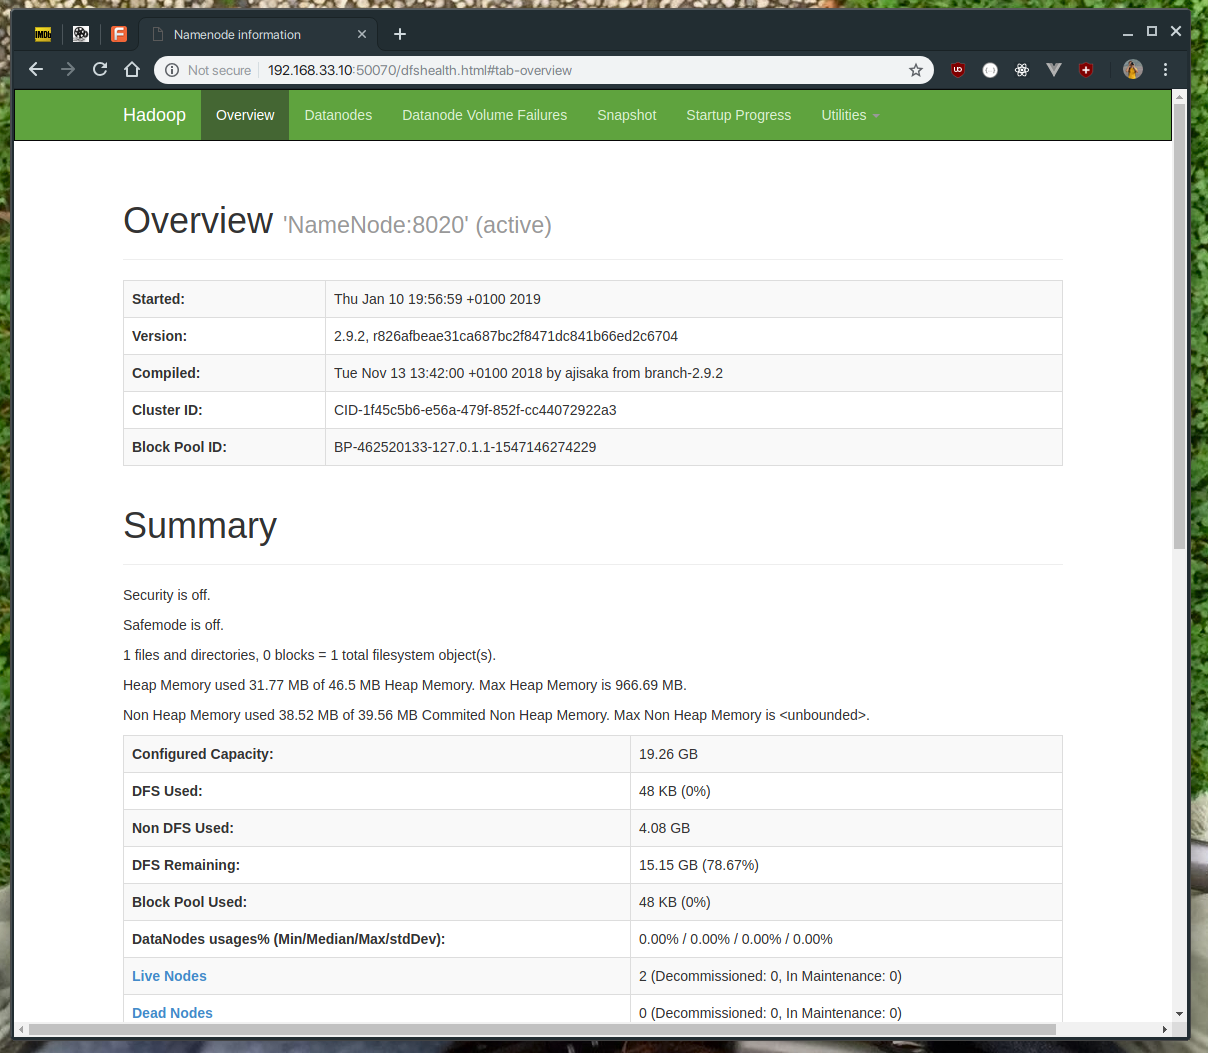
\includegraphics[scale=0.5]{./namenode-overview.png}
\caption{Pregled Namenode vozlišča}
\label{nno}
\end{center}
\end{figure}

\begin{figure}
\begin{center}
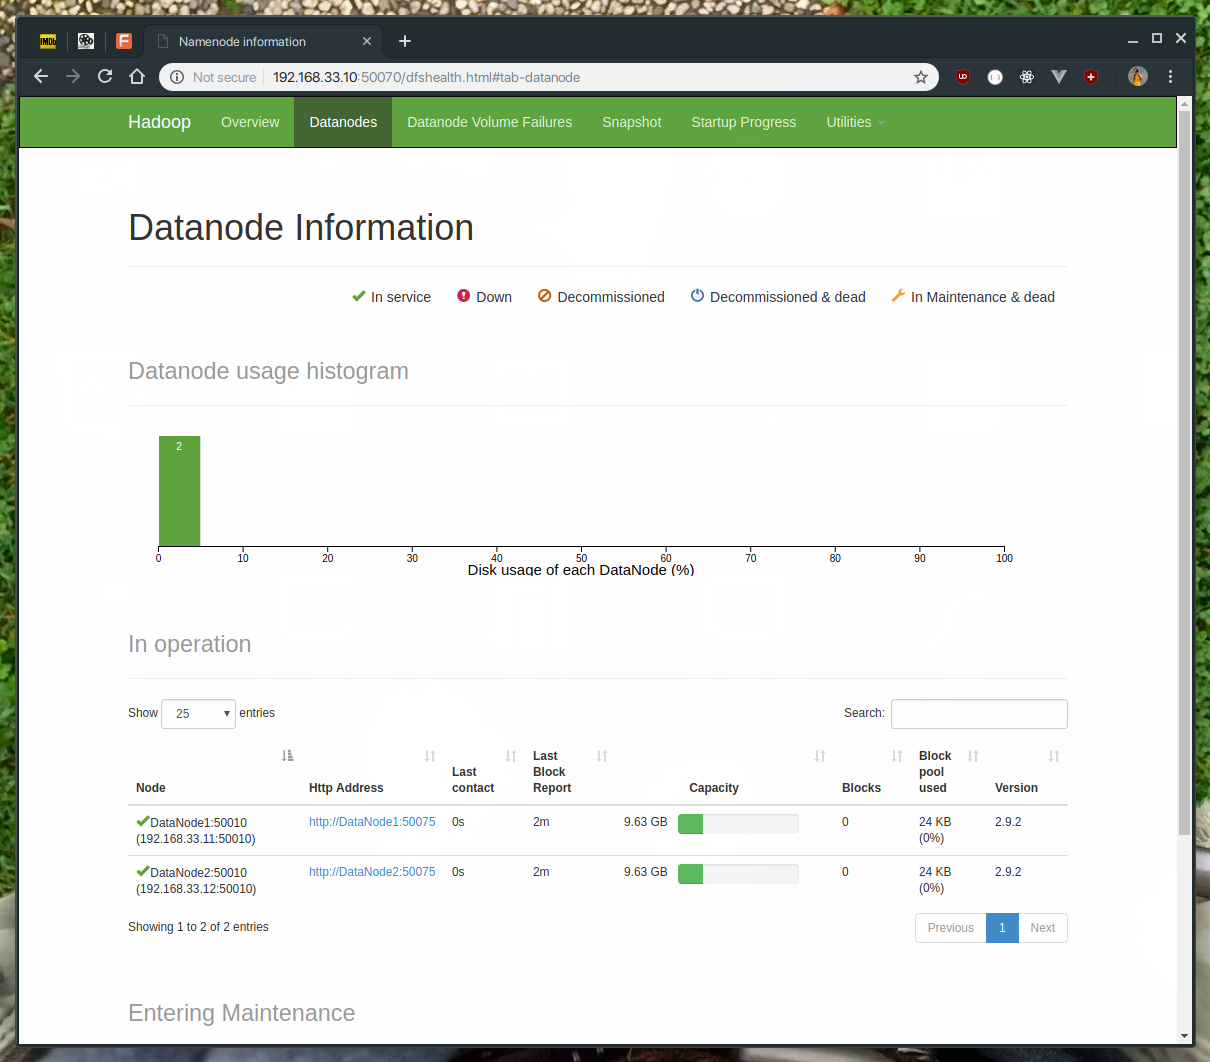
\includegraphics[scale=0.5]{./namenode-datanodes.png}
\caption{Pregled nad Datanode vozlišči, v našem primeru 2}
\label{nnd}
\end{center}
\end{figure}

\begin{figure}
\begin{center}
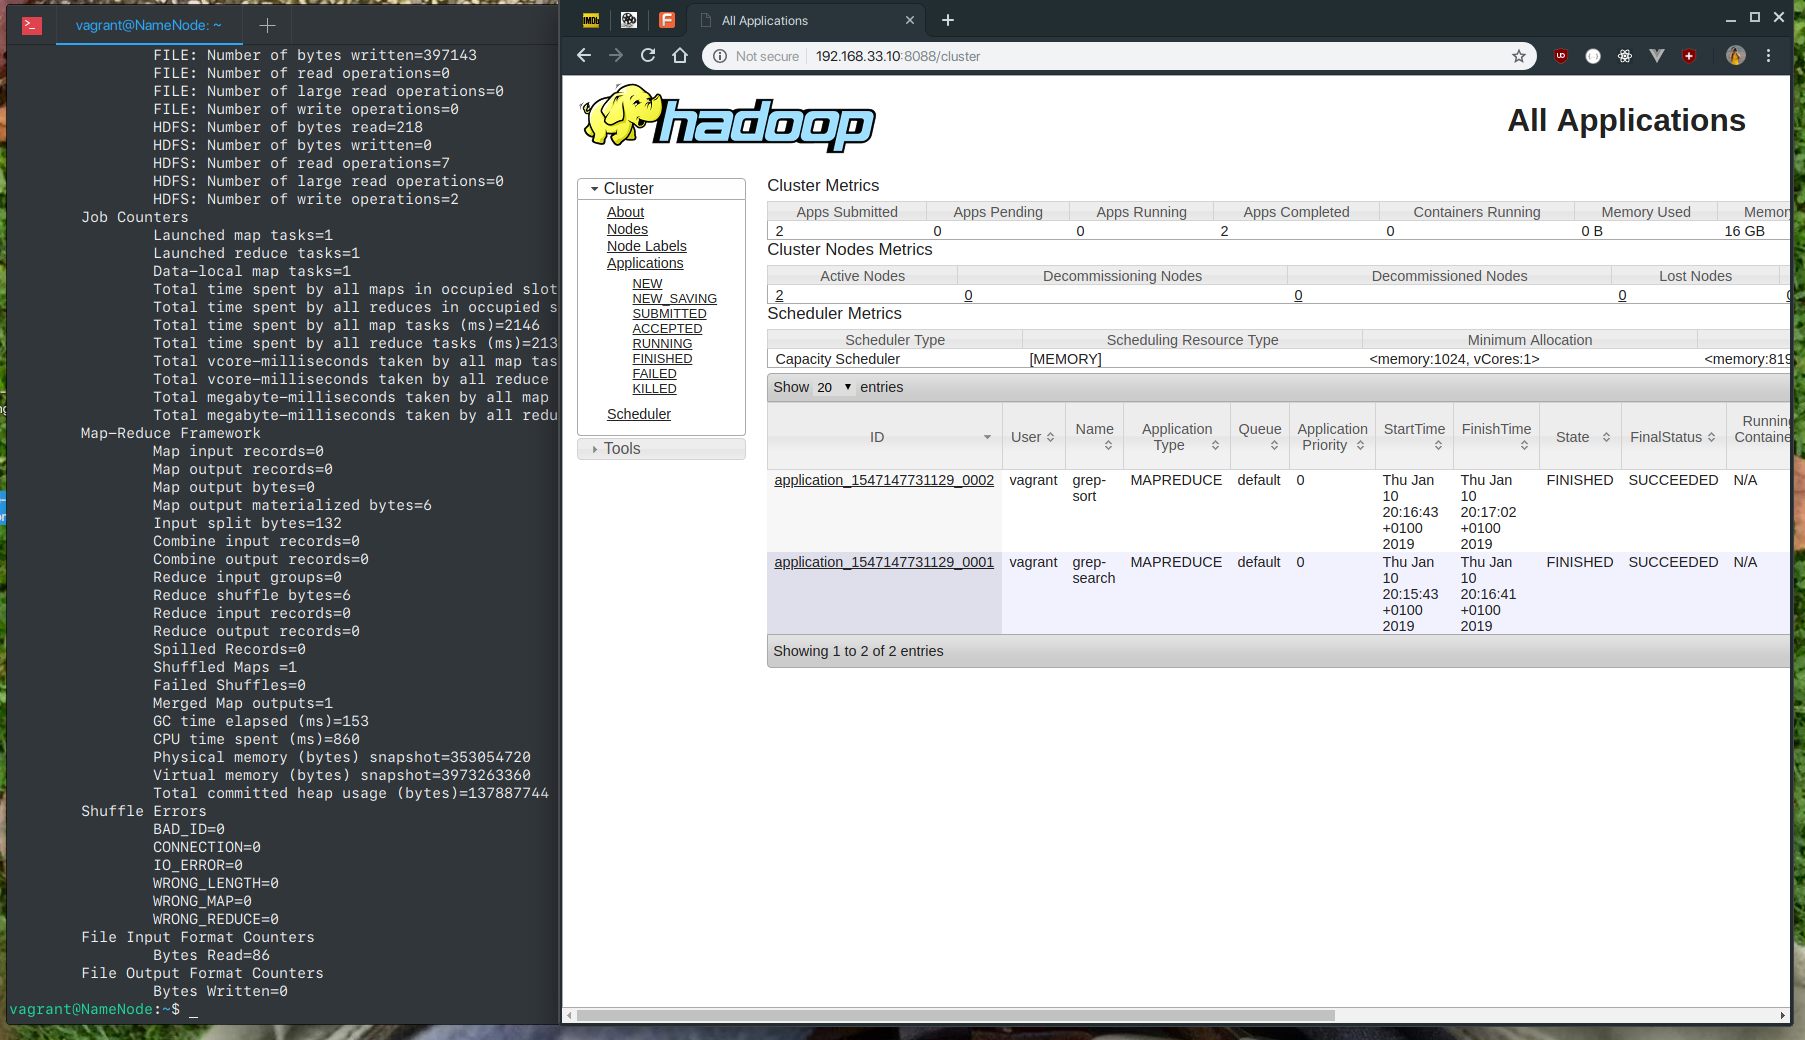
\includegraphics[scale=0.35]{./mapreduce-example.png}
\caption{Zagon primera MapReduce programa}
\label{mre}
\end{center}
\end{figure}


\section{Izjava o izdelavi domače naloge}
Domačo nalogo in pripadajoče programe sem izdelal sam.

\end{document}
